\documentclass[12pt,a4paper]{article}
\usepackage[utf8]{inputenc}
\usepackage[T1]{fontenc}
\usepackage[french]{babel}
\usepackage{graphicx}
\usepackage{float}
\usepackage{hyperref}

\title{Titre} 
\author{Panchalingamoorthy Gajenthran} 
\date{Date}

\begin{document}
%\maketitle{}
\begin{titlepage}
	\centering
	{\scshape\LARGE Université Paris 8 \par}
	\vspace{1cm}
	{\scshape\Large Cours de Traitement de Signal et d'Image \par}
	\vspace{4.5cm}
	{\huge\bfseries FaceWorker\par}
	\vspace{1cm}
	{\Large\itshape Panchalingamoorthy Gajenthran \par}
	{\Large\itshape Hu Sacha \par}
	\vfill
	
	{\large \today\par}
\end{titlepage}

\tableofcontents

% Use \texttt{} for commands
% Use \textit{} for files
% Use  \underline for notes
% Use \includegraphics for images:
    % \begin{figure}[H]
    % \centering
    % \includegraphics[scale=0.5]{image.png}
    % \caption{Nom de l'image}
    % \end{figure}
% Use \href{http://www.sharelatex.com}{Nom du lien} for links
% Use \item for lists with bullets:
     % \begin {itemize}\renewcommand {\labelitemi }{$\bullet $}
     % \item 
     % \end {itemize}
     

\section{Introduction} 
L'application FaceWorker est capable d’appliquer des filtres à une photo, de reconnaitre un visage sur une photo, ou même de reconnaître une personne en video en temps réel.
\newline
L’application se présente ainsi : 3 boutons pour accéder aux trois fonctionnalités principales que propose FaceWorker : FaceFilter, IRecognition (Eigenfaces) ou VRecognition (reconnaissance faciale en temps réel). 
\newline
La première permet de charger une image, de sélectionner un ou plusieurs filtres via une interface très intuitive qui propose de nombreux filtres dans un menu déroulant et accessibles via des boutons sur le côté droit de l’image. Lorsque l’image est chargée, on peut directement visualiser les modifications apportées sur l’image. Lorsque les modifications sont faites, on peut sauvegarder l’image.
\newline
La deuxième, permet de charger une image et de détecter le visage puis en parcourant une base de données de visages pré-enregistrées, reconnaitre à qui appartient cette photo. 
 \newline
 La dernière option, est malheureusement encore en cours d’implémentation car elle s’est avérée plus complexe que prevue. Nous allons tout de même expliquer son fonctionnement. Elle permet de reconnaître en temps réel le visage d’une personne et de lui associer un nom.
 \newline
 Toute cette interface a été réalisée à l’aide de la toolbox Guide qui permet de créer de très bonnes interfaces graphiques.
 
\section{Filtres}
Cette partie de notre application permet d’appliquer toutes sortes de filtres. Nous avons implémenté à la main, 17 filtres différents dont les filtres passe haut, passe bas ou des filtres utilisant les histogrammes mais pas seulement (une liste exhaustive est donnée plus bas). Il est également possible de cumuler différents filtres et ainsi de rajouter un second filtre par-dessus un premier filtre. Enfin, lorsque tous les filtres souhaités ont été rajoutés, il est possible d’enregistrer l’image, ce qui crée un nouveau fichier utilisable par la suite. 
\newline
L'ensemble des filtres se trouvent dans le fichier \textit{fwFilter.m}. A noter que tous les fichiers métiers comporteront le préfixe \texttt{fw} pour FaceWorker.
\newline
Il existe 17 filtres différents dans notre application : nuance de gris, binaire, complément binaire, égalisation d’histogramme, Sobel, Sepia, Prewitt, luminosité, Laplacien, Sharpen, moyenneur, médian, inversion de couleurs, tourbillon, bilatéral, interpolation bilinéaire et miroir.

\subsection{Nuance de gris}
Ce filtre (\texttt{applyGrayscale}) permet de faire passer une image en couleur en une image composée de nuance de gris. D'abord, nous vérifierons si l'image sélectionnée est bien une image en couleur puis appliquer notre algorithme. Matlab possède déjà la fonction \texttt{rgb2gray} mais nous avons décidé de créer la notre qui ajoute la vérification précédemment expliquée.

\begin{figure}[H]
\centering
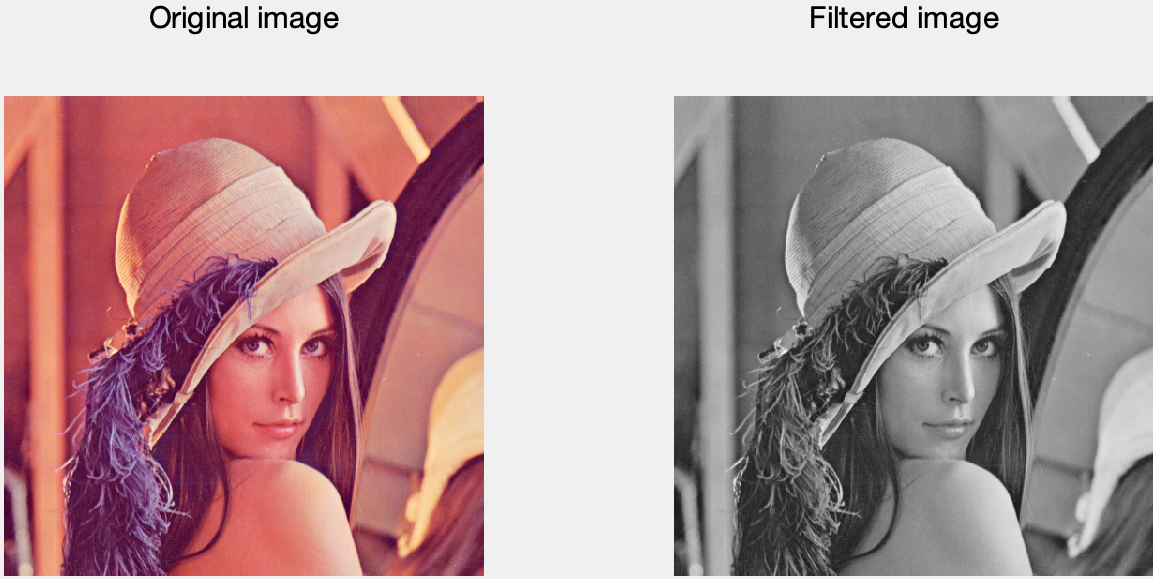
\includegraphics[scale=0.5]{img/grayscale}
\caption{Nuance de gris}
\end{figure}
    
\subsection{Egalisation d'histogramme}
L'égalisation d'histogramme (\texttt{applyHistEq}) va nous permettre d'ajuster le contraste d'une image en s'aidant de l'histogramme de celle-ci. Pour réaliser ce filtre, trois étapes sont à noter : la création de l'histogramme de l'image, le calcul de l'histogramme cumulée grâce à l'histogramme créé précédemment et enfin l'application de l'égalisation de l'histogramme pour chaque pixel de l'image.

\begin{figure}[H]
\centering
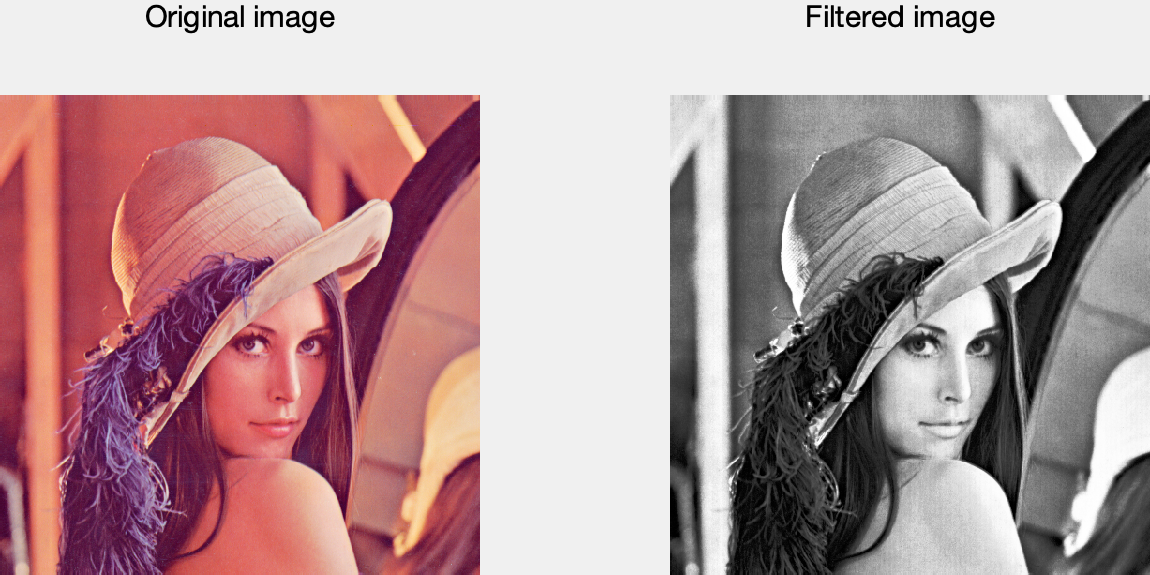
\includegraphics[scale=0.5]{img/heq}
\caption{Egalisation d'histogramme}
\end{figure}

\subsection{Sobel}
Le filtre de Sobel (\texttt{applySobel}) est un filtre de passe-haut car il permet de détecter les contours de l'image en utilisant des matrices de convolution. Ainsi on obtiendra le gradient X pour une image I et le gradient Y pour une image I. La combinaison des deux gradients permet d'obtenir une approximation de la norme du gradient à l'aide de la formule suivante : \texttt{$ G = sqrt( Gx\wedge2 + Gy \wedge2 ); $}. Notre algorithme est plutôt lent vu qu'il s'agit de faire des boucles imbriquées les unes sur les autres et également plusieurs calculs (c'est pour cela que nous avons remplacé \texttt{$ G = sqrt( Gx\wedge2 + Gy \wedge2 ); $} par \texttt{$ G = abs(Gx) + abs(Gy); $} afin de réduire le temps d'exécution). Une alternative aurait été d'utiliser la méthode \texttt{conv2} offerte par Matlab.

\begin{figure}[H]
\centering
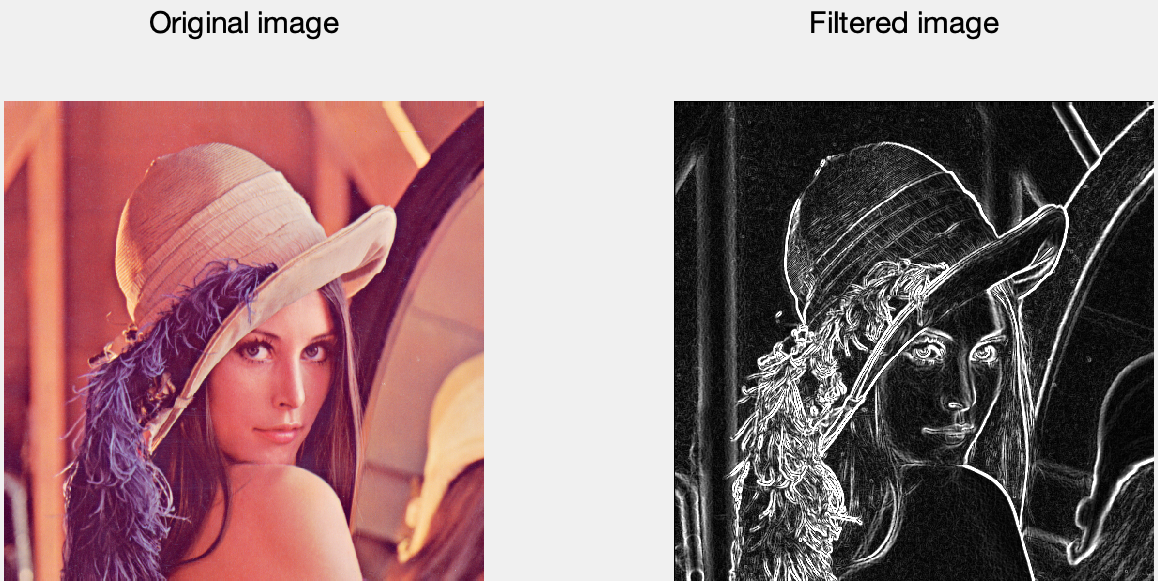
\includegraphics[scale=0.5]{img/sobel}
\caption{Filtre de Sobel}
\end{figure}

\subsection{Prewitt}
De la même manière que le filtre de Sobel, le filtre de Prewitt (\texttt{applyPrewitt}) va nous permettre de detecter les contours de l'image. Seulement, les matrices qui vont convoluer vont être différentes des matrices du filtre de Sobel donc le rendu concernant les contours seront différents comme nous pouvons le voir dans l'image ci-dessous.

\begin{figure}[H]
\centering
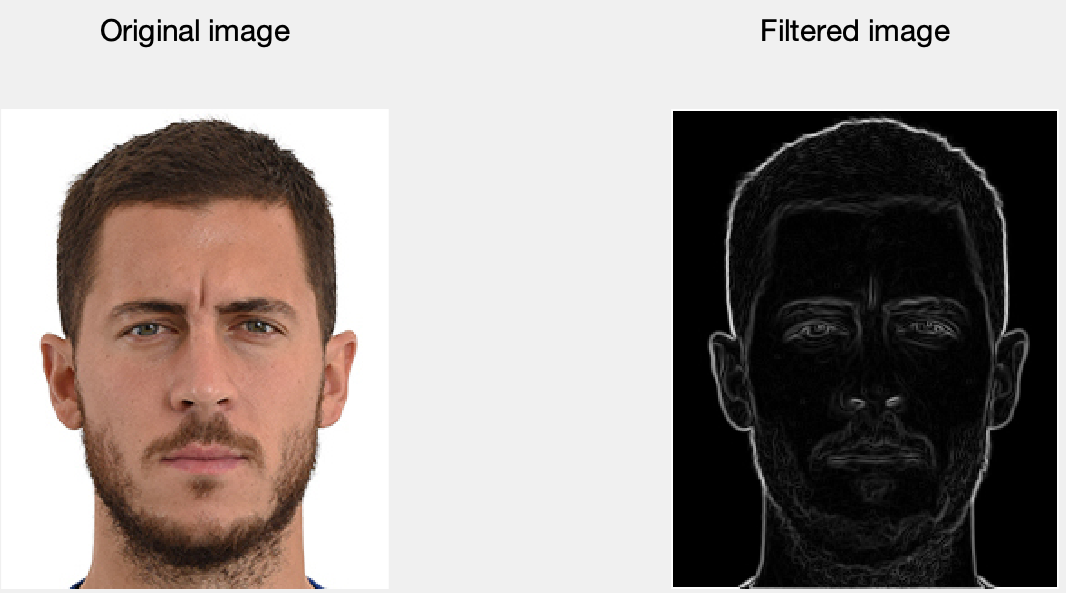
\includegraphics[scale=0.5]{img/prewitt}
\caption{Filtre de Prewitt}
\end{figure}

\subsection{Laplacien}
Exactement comme les deux autres cités  auparavant (Sobel et Prewitt), ce filtre (\texttt{applyLaplacian}) est également un filtre passe-haut. 

\begin{figure}[H]
\centering
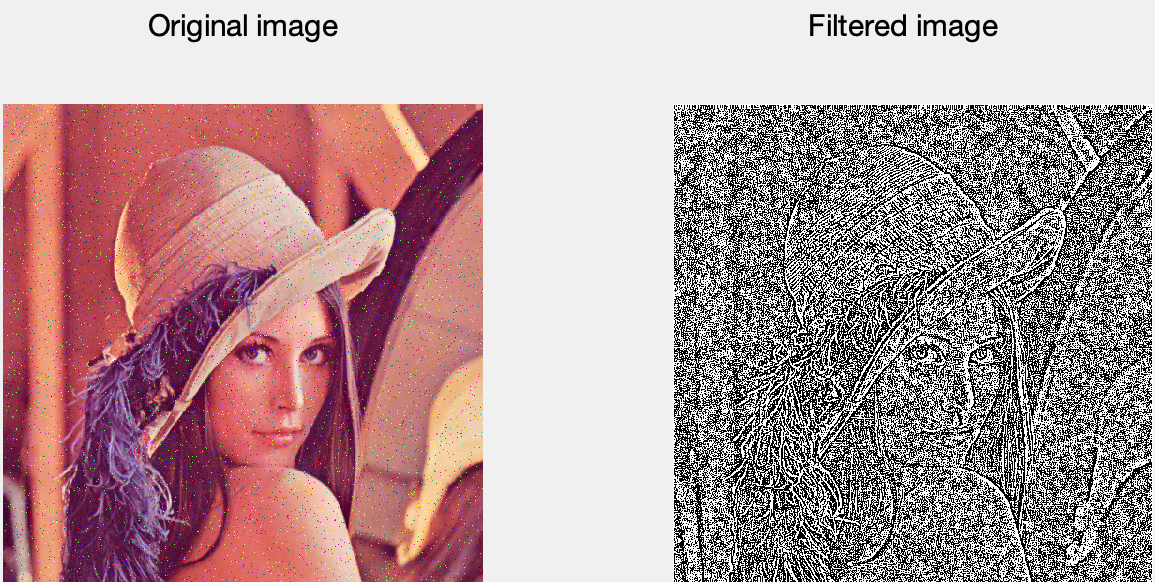
\includegraphics[scale=0.5]{img/laplacien}
\caption{Filtre laplacien}
\end{figure}

\subsection{Sharpen}
Pour finir sur les filtres passe-haut, le filtre Sharpen permet également de calculer le contours en utilisant des gradients différents.

\begin{figure}[H]
\centering
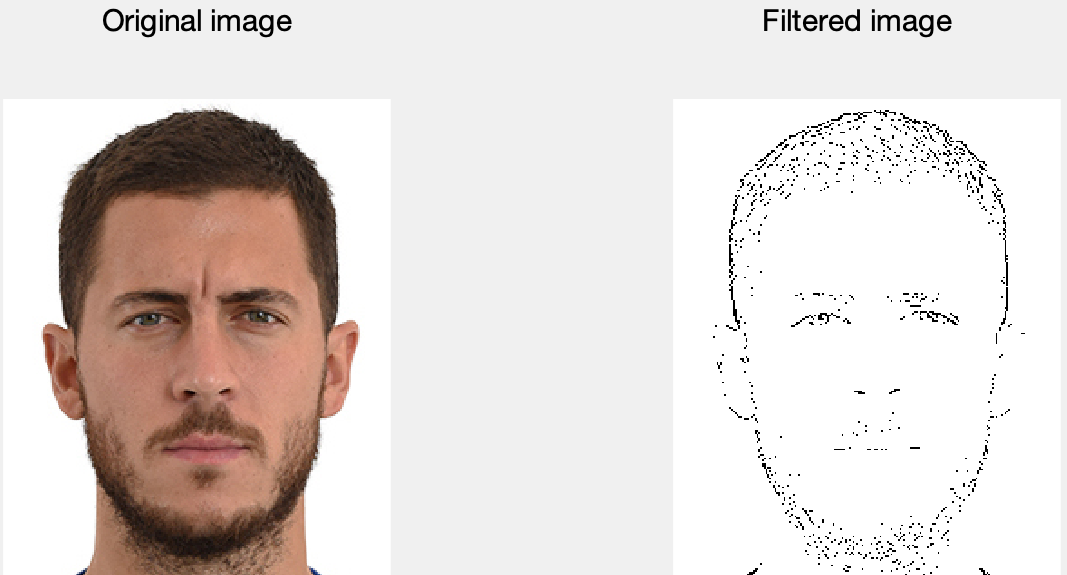
\includegraphics[scale=0.5]{img/sharpen}
\caption{Filtre Sharpen}
\end{figure}

\subsection{Moyenneur}
Le filtre moyenneur (\texttt{applyAverage}) est un filtre de passe-bas : en effet, il réduit les détails (mais aussi le bruit) et permet d'obtenir une image plus lisse. Il consiste à remplacé le pixel sélectionné par la moyenne de ses pixels voisins. Une amélioration de ce filtre serait le filtre Gaussian car il offre un meilleur lissage et moins de bruit.

\begin{figure}[H]
\centering
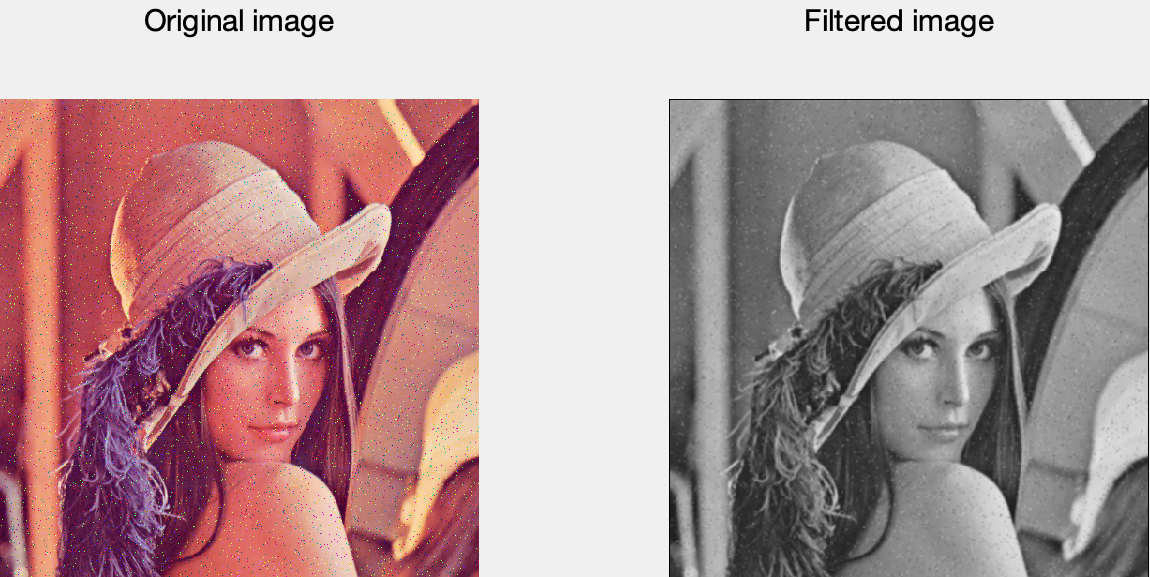
\includegraphics[scale=0.5]{img/average}
\caption{Filtre moyenneur}
\end{figure}

\subsection{Médian}
Le filtre médian (\texttt{applyMedian}) est une opération non linéaire, plutôt utilisé pour réduire les bruits d'une image. Le principe est assez simple : sur un pixel sélectionné, on applique la médiane de tous les pixels voisins.

\begin{figure}[H]
\centering
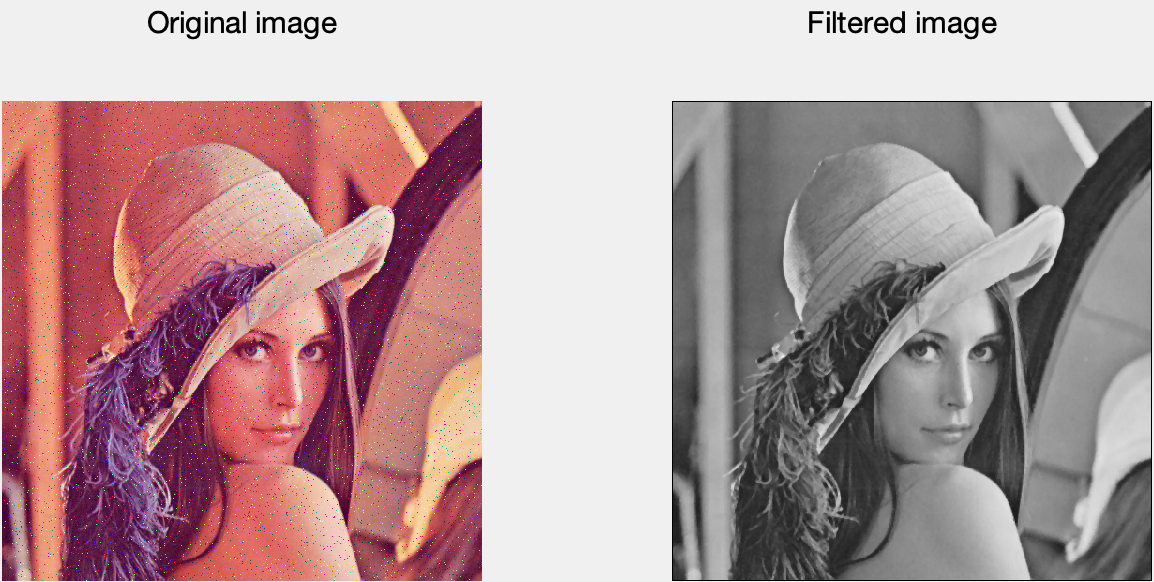
\includegraphics[scale=0.5]{img/median}
\caption{Filtre médian}
\end{figure}

\subsection{Inversion des couleurs}
Comme son nom l'indique, ce filtre  (\texttt{applyInvert}) va nous permettre d'inverser les couleurs d'une image. L'implémentation de l'inversion des couleurs est assez il suffit de prendre la valeur maximale de chaque couleur à savoir 255 et de la soustraire par la couleur actuelle. 

\begin{figure}[H]
\centering
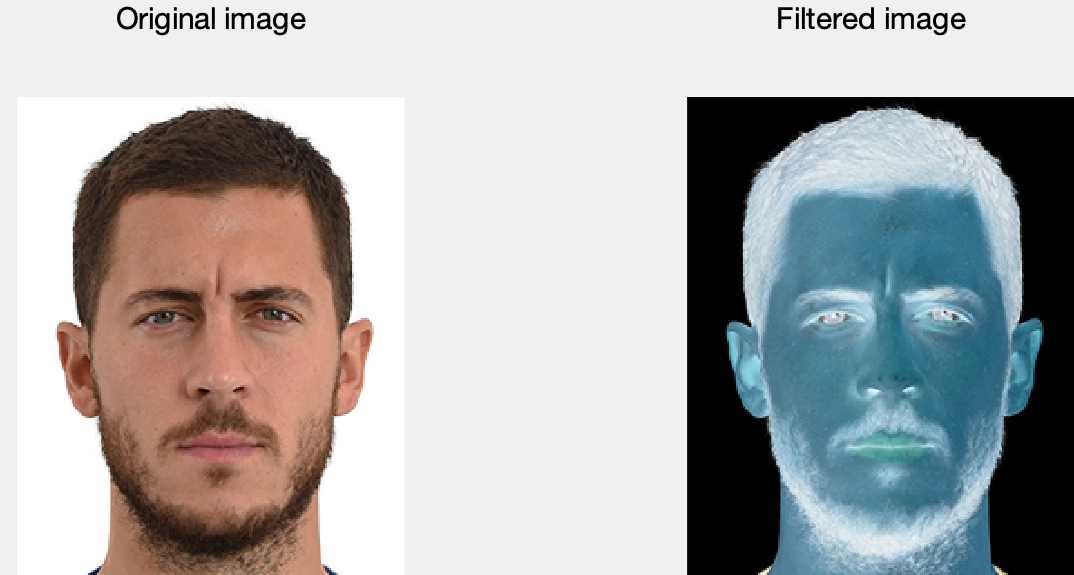
\includegraphics[scale=0.5]{img/invert}
\caption{Inversion des couleurs}
\end{figure}

\subsection{Sepia}
Le filtre Sépia (\texttt{applySepia}) va nous permettre d'apporter une teinte plus ancienne à notre image et offrir une photo plus vintage (avec une domination de la couleur jaune). Pour chaque couleur de l'image, on va additionner les 3 couleurs (RGB) en appliquant un coefficient différent pour chaque couleur. 
\newline
Par exemple pour le nouveau rouge du Sépia \texttt{NR = (R * 0.393) + (G * 0.769) + (B * 0.189);}

\begin{figure}[H]
\centering
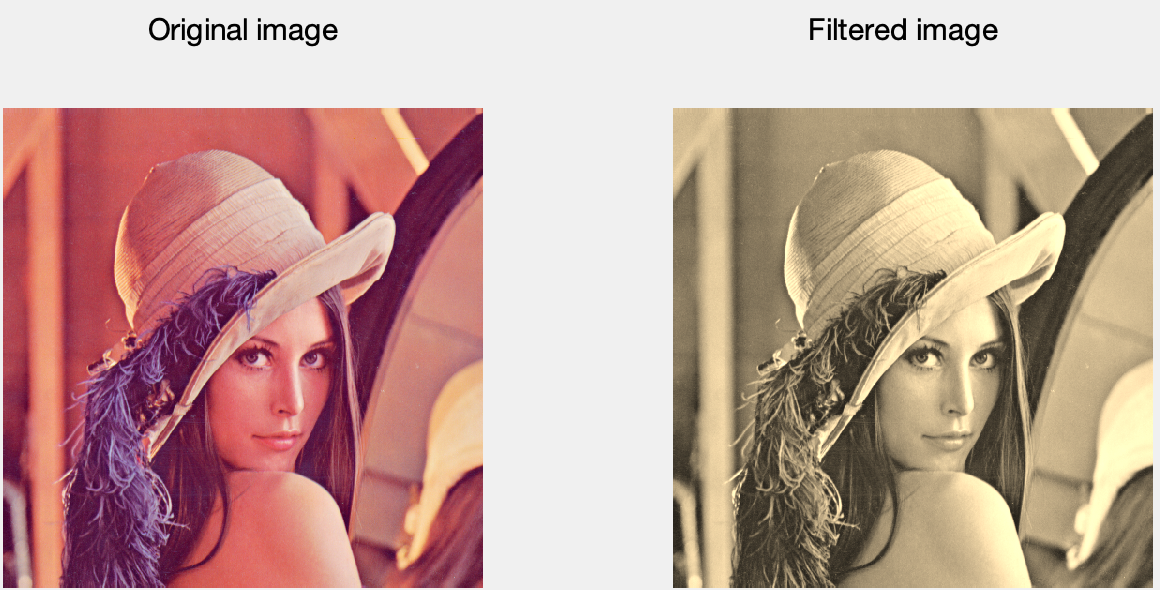
\includegraphics[scale=0.5]{img/sepia}
\caption{Filtre Sépia}
\end{figure}

\subsection{Luminosité}
Améliorer la luminosité (\texttt{applyBrightness}) se réalise de manière assez simple : il suffit de décaler l'histogramme \texttt{I'(i, j) = I(i, j) + b} où \texttt{b} est le facteur de décalage. Dans notre application, pour gérer le mieux possible la luminosité de l'image, un slide-bar est mis à disposition représentant le facteur de décalage (entre 0 et 100)

\begin{figure}[H]
\centering
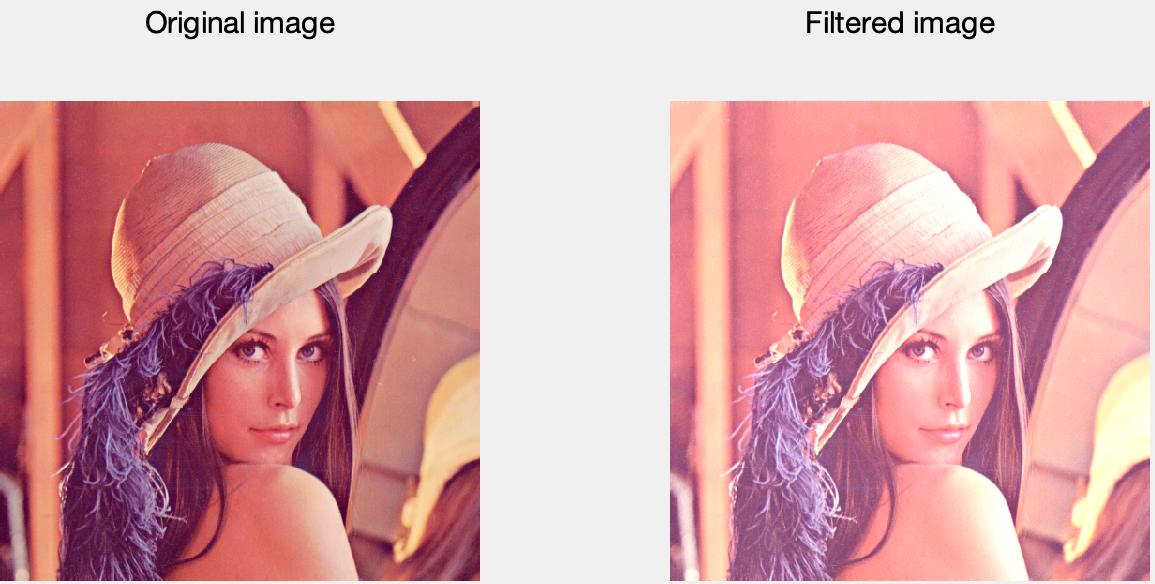
\includegraphics[scale=0.5]{img/brightness}
\caption{Luminosité}
\end{figure}

\subsection{Tourbillon}
Le filtre Tourbillon (\texttt{applySwirl}) va créer une sorte de spirale déformant l'image en plusieurs morceaux donnant l'impression que l'image se fait aspirer par un tourbillon. On utilisera les fonctions \texttt{cos} et \texttt{sin} pour réaliser ce filtre. Comme pour la luminosité, on bénéficiera d'un slide-bar gérant le degré de transformation de l'image.

\begin{figure}[H]
\centering
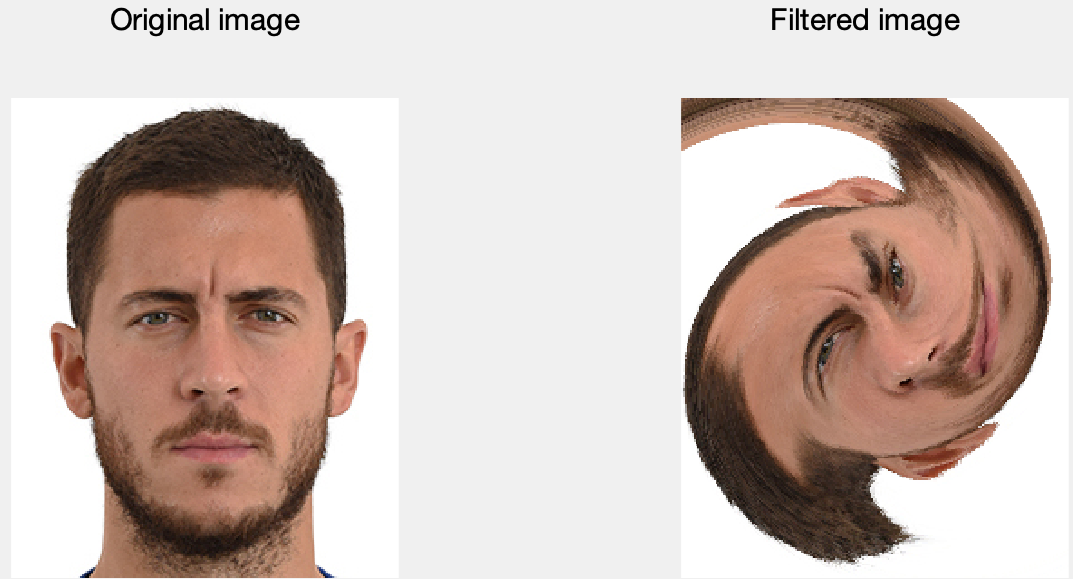
\includegraphics[scale=0.5]{img/swirl}
\caption{Filtre swirl}
\end{figure}

\subsection{Bilateral}
Le filtre bilateral (\texttt{applyBilateralRGB}) est un filtre de passe-bas permettant de réduire les bruits tout en rendant l'image plus lisse. Il peut être utilisé pour transformer une image réel en une image en cartoon par exemple.

\begin{figure}[H]
\centering
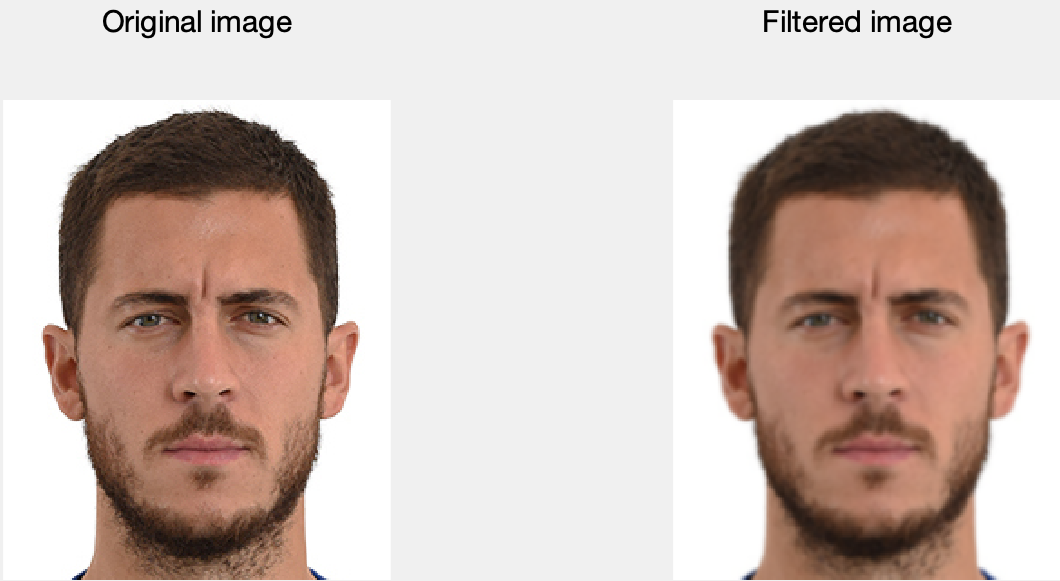
\includegraphics[scale=0.5]{img/bilateral}
\caption{Filtre bilatéral}
\end{figure}

\subsection{Interpolation bilinéaire}
L'interpolation bilinéaire \texttt{applyInterpolationB} consiste à agrandir les dimensions de l'image par copie de pixels. Le principe est assez simple, chaque pixel de la nouvelle image sera de la forme : \texttt{I'(i, j) = I(i/scale, j/scale)} où \texttt{scale} correspond au coefficient séparant l'échelle de départ et la nouvelle échelle. On peut très bien créer deux \texttt{scale} différents (un pour la colonne et un autre pour la ligne).

\begin{figure}[H]
\centering
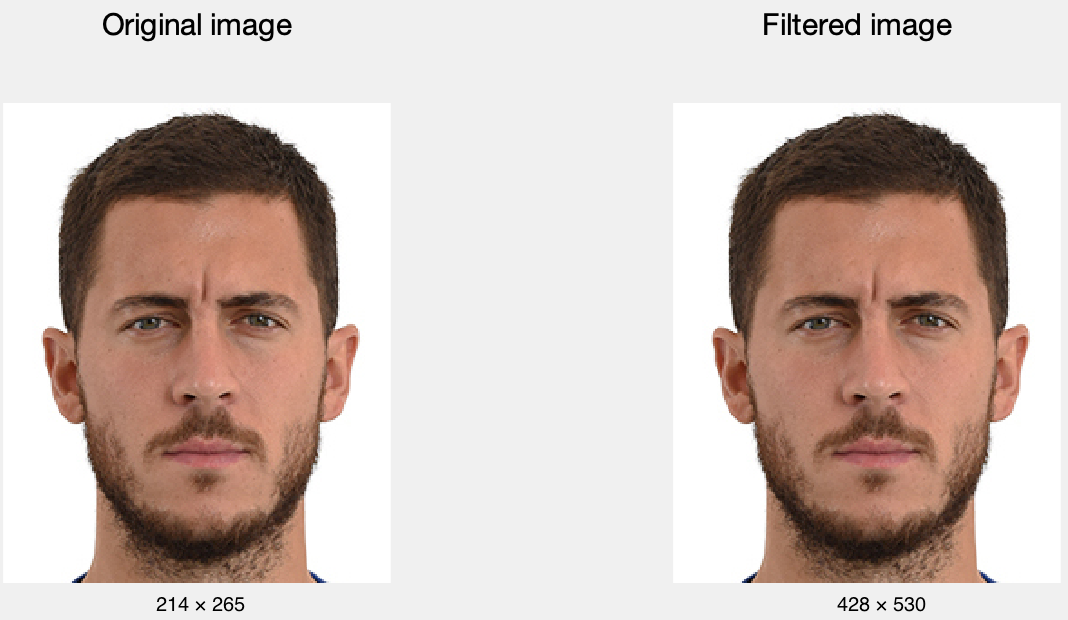
\includegraphics[scale=0.5]{img/interpolation}
\caption{Interpolation bilinéaire}
\end{figure}

\subsection{Rotation}
Le filtre de rotation \texttt{applyRotation} permet de réaliser une rotation de l'image selon un angle de rotation \texttt{a} autour de son centre en appliquant pour chaque pixel la formule suivante :
\newline
\texttt{x = W /2 + (x0 - W /2) * cos(a) - (y0 - H/2) * sin(a)}
\newline
\texttt{y = H/2 + (y0 - H/2) * cos(a) + (x0 - W/2) * sin(a)}
\newline
Notre formule est légèrement différente de celle-ci mais réalise la même rotation.

\begin{figure}[H]
\centering
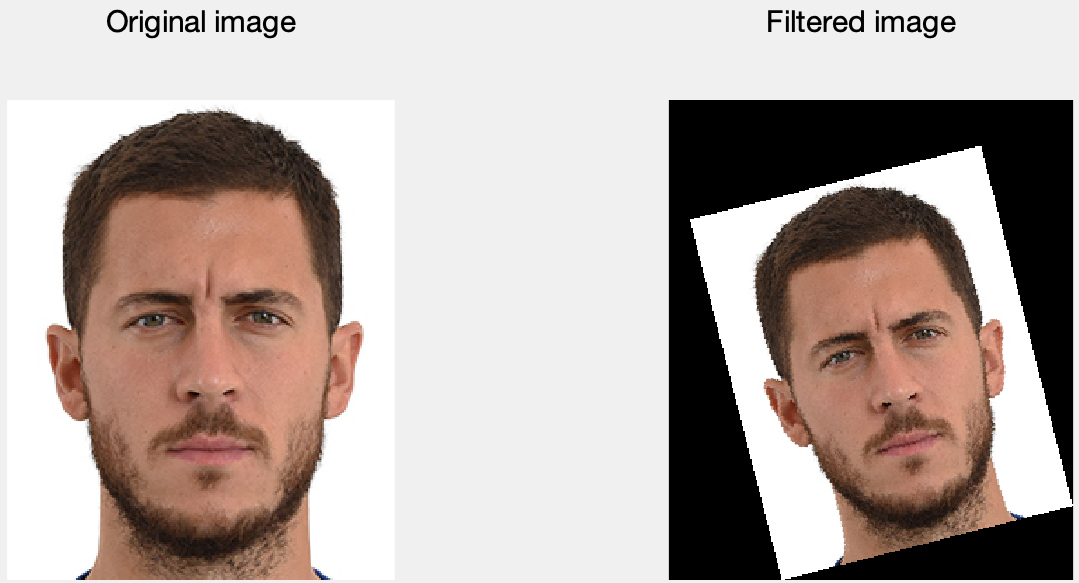
\includegraphics[scale=0.5]{img/rotate}
\caption{Rotation}
\end{figure}

\subsection{Miroir}
Le miroir \texttt{applyMirror} permet de retourner l'image de la gauche vers la droite. Concernant l'implémentation, soient \texttt{w(j) = 1 + j} et \texttt{w'(j) = width - j}, on a alors \texttt{I'(i, w(j)) = I(i, w'(j))}

\begin{figure}[H]
\centering
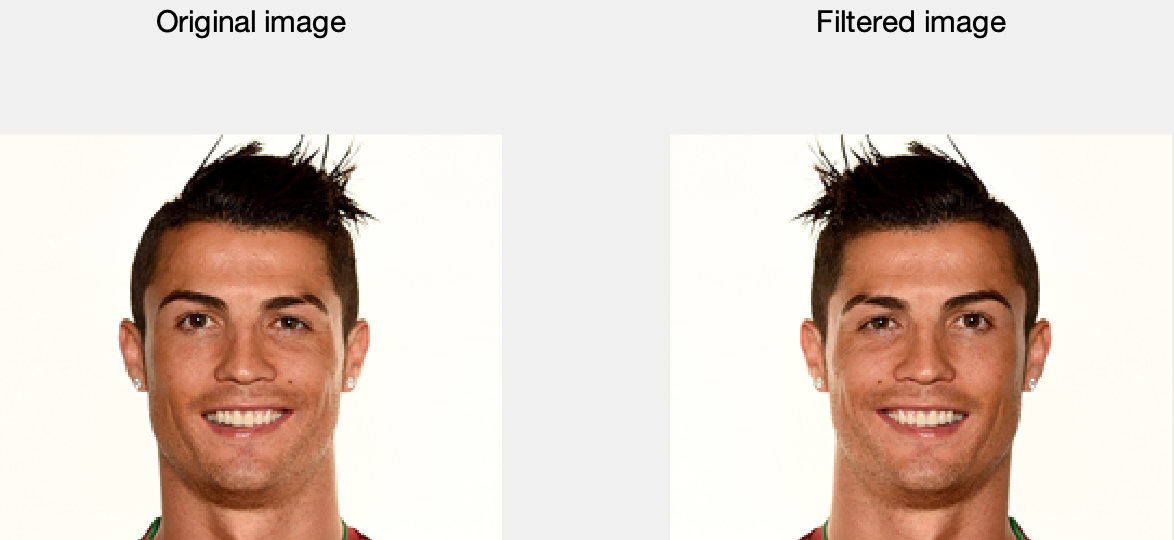
\includegraphics[scale=0.5]{img/mirror}
\caption{Filtre Miroir}
\end{figure}

\subsection{Binaire}
Le filtre binaire (\texttt{applyBinary}) consiste à représenter l'image avec seulement des valeurs composées de 0 et de 1 et donc une image composée de noir et blanc. Pour cela, on transforme l'image en gris si ce n'est pas le cas, puis on calcule moyenne de la valeur de gris (qui sera notre seuil) et enfin toutes les valeurs au-dessus de ce seuil seront représentées par des 1 et le reste par des 0.

\begin{figure}[H]
\centering
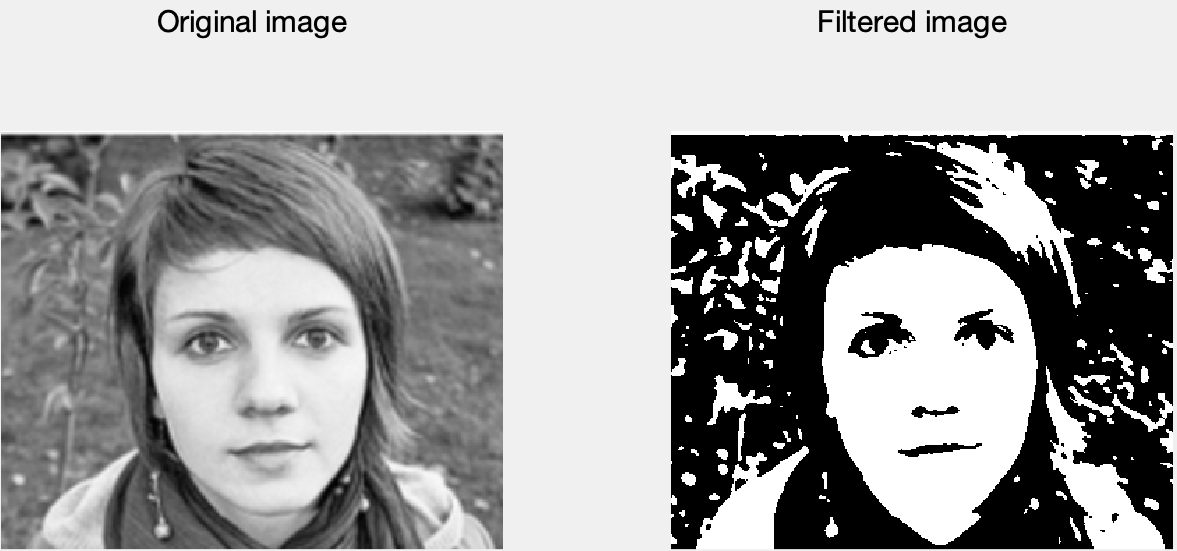
\includegraphics[scale=0.5]{img/binary}
\caption{Filtre binaire}
\end{figure}

\subsection{Complément binaire}
En admettant que notre image est en binaire (sinon on applique le filtre binaire vu ci-dessus), on peut ainsi appliquer son complément (\texttt{applyComplementBinary}), c'est-à-dire transformer tout ce qui est en noir, en blanc et tout ce qui est en blanc, en noir, ce qui revient donc à inverser les 0 en 1 et vice-versa.

\begin{figure}[H]
\centering
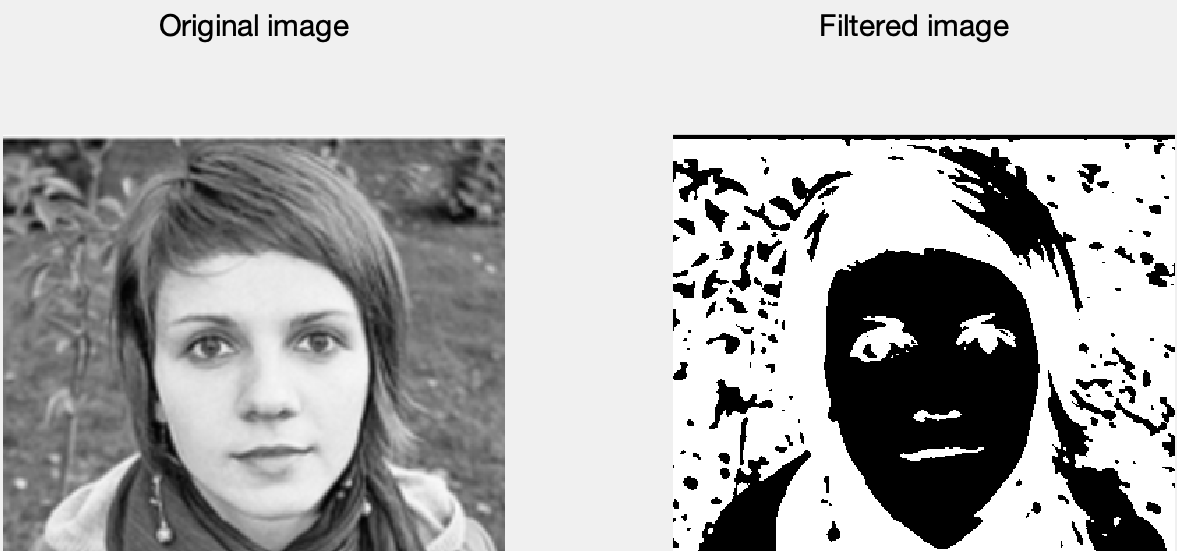
\includegraphics[scale=0.5]{img/complement-binary}
\caption{Filtre complément binaire}
\end{figure}


\section{IRecognition : Eigenfaces}
Cette fonctionnalité permet de reconnaitre une image parmi une base de données à l'aide de la méthode Eigenfaces. Les eigenfaces sont un ensemble de vecteurs propres utilisés dans le domaine de la vision artificielle afin de résoudre le problème de la reconnaissance du visage humain. Le recours à des eigenfaces pour la reconnaissance a été développé par Sirovich et Kirby (1987) et utilisé par Matthew Turk et Alex Pentland pour la classification de visages. Cette méthode est considérée comme le premier exemple réussi de technologie de reconnaissance faciale. Ces vecteurs propres sont dérivés de la matrice de covariance de la distribution de probabilité de l'espace vectoriel de grande dimension des possibles visages d'êtres humains (source: Wikipedia). 
\newline
Cette méthode va permettre d'identifier le visage en analysant l'ensemble du visage, on parle alors d'analyse en composant principale (PCA) se différenciant ainsi des méthodes géométriques ou locales qui eux se concentrent sur les signes/marques du visage (et qui peuvent parfois paraître imprécises). La méthode Eigenfaces est un algorithme plutôt simple à implémenter et efficace : elle présente un bon taux de réussite (évidemment plus la base de données est grande, plus le taux de réussite est significatif).
\newline
Les fonctions concernant Eigenfaces se trouvent dans le fichier \textit{fwEigen.m} : nous avons les fonctions principales \texttt{fwEigen} qui correspond au constructeur de la classe et qui charge la base de données d'apprentissage (le dossier \textit{Dataset}) et une image à reconnaître (quelques images exemples sont données dans le dossier \textit{Testset}), et \texttt{recognize} qui s'occupe de reconnaître le visage demandé dans la base de données.

\subsection{Dataset : base de données d'apprentisage}
Pour les données d'apprentissage, nous avons collecté les images du laboratoires AT\&T pour avoir une base de données assez conséquente, puis par dessus nous avons rajouter d'autres images sous différents formats afin d'être capable de traiter tous les cas.
Ainsi, la BDD contient 43 dossiers où chaque dossier comporte 10 images.
\newline
Les fonctions \texttt{loadFaceDatabase} et  \texttt{loadFaceDatabaseCD} permettent de charger la base de données et d'exploiter un ensemble d'image sous forme de matrice. Vu que \texttt{loadFaceDatabaseCD} présente quelques inconvénients du fait qu'elle sollicite l'utilisation de \texttt{cd} (change directory), nous allons plutôt privilégier \texttt{loadFaceDatabase}. 
\newline
Pour chaque image dans la base de données, on se chargera de vérifier quelques critères importants. Ce programme ne prend que des images au format \textit{.pgm}, donc il faudra faire gaffe au format des fichiers. L’image doit être d’une certaine taille : 92*112. Cependant, si elle n’est pas conforme à ces dimensions, elle sera juste redimensionnée (à l'aide de la fonction \texttt{imresize} en lui précisant la taille souhaitée) afin que l’on puisse continuer. Afin d’utiliser la méthode Eigenfaces, il faut également que l’image soit en nuances de gris (à l'aide de la fonction \texttt{rgb2gray}, cette fois-ci pas celle que nous avons créé afin de ne pas avoir de soucis par rapport au temps). Evidemment, si ce n’est pas déjà le cas, nous transformons l’image en nuances de gris. Dans un premier temps, nous voulions utiliser la fonctionnalité de Matlab permettant de rogner l’image (avec \texttt{imcrop} et \texttt{vision.CascadeObjectDetector} en ne conservant que le visage, partie qui nous intéresse, mais celle-ci découpait un visage trop réduit et retirait certains traits de visage comme le menton ou les cheveux. Nous avons donc testé sans rogner et cela fonctionnait bien mieux. Donc nous devons faire en sorte que le visage soit correctement cadré. De plus, il faut également faire attention aux fichiers cachés (comme les fichiers \textit{.DS\_Store} pour les utilisateurs de MacOS)

\subsection{Testset : les images à tester}
Une fois, la base de données chargée, la fonction \texttt{loadTestImage} va maintenant choisir une image en vérifiant également certains critères. Si un format d’image autre que \textit{.pgm} est chargée, une copie de cette image sera créée, cette fois au format \textit{.pgm}, et on utilise par la suite cette image (on s'occupera également de la suppression de ce fichier créé une fois l'application fermée). Pour cela, la fonction \texttt{convert2pgm} s'occupe de récupérer le nom du fichier et les détails le concernant (chemin et extension) en utilisant la fonction \texttt{fileparts} et on vérifie si l'extension est bien en \textit{.pgm}. Si ce n'est pas le cas, on remplace l'extension du fichier par \textit{.pgm} à l'aide de \texttt{strrep} et on crée un nouveau fichier tout en modifiant la variable \texttt{fileCreated} à \texttt{1} pour pouvoir supprimer ce fichier à la fermeture de l'application. 
\newline
Puis, on se contente aussi de vérifier si l'image en question est en nuance de gris, avec des dimensions correctes (92*112) et on se chargera de la mettre en \texttt{uint8} pour pouvoir l'utiliser lors de la reconnaissance. Toutes ces vérifications et transformations se trouve dans la fonction \texttt{transformImage}.

\subsection{Reconnaissance et identification}
Apres cela, nous appliquons l’algorithme de Eigenfaces. Pour cela, il faut tout d'abord commencer par trouver le visage moyen de notre base de données à l'aide de la fonction \texttt{mean}, puis soustraire ce visage moyen des visages de la base de données d'apprentisage ce qui nous permet de savoir les caractéristiques propres de chaque visage qu'on appelle \texttt{eigenfaces} et qu'on trouvera à l'aide de la fonction \texttt{eig} (qui est l'équivalent de \texttt{spec} en SciLab). Et enfin, on parcourt toutes les images de la base de données en comparant le poids de chaque image de la base de données calculée avec \texttt{eig} avec celui de l'image selectionné. L'image de la base de données ayant le poids le plus faible correspond à l'image qui a la plus forte ressemblance avec l'image sélectionnée. Cette photo est ensuite affichée. Par la suite nous aimerions que chaque image de la base de donnée soit liée a un prénom, de manière a ce que lorsqu’on reconnait une photo, on puisse directement afficher le nom de la personne.

\begin{figure}[H]
\centering
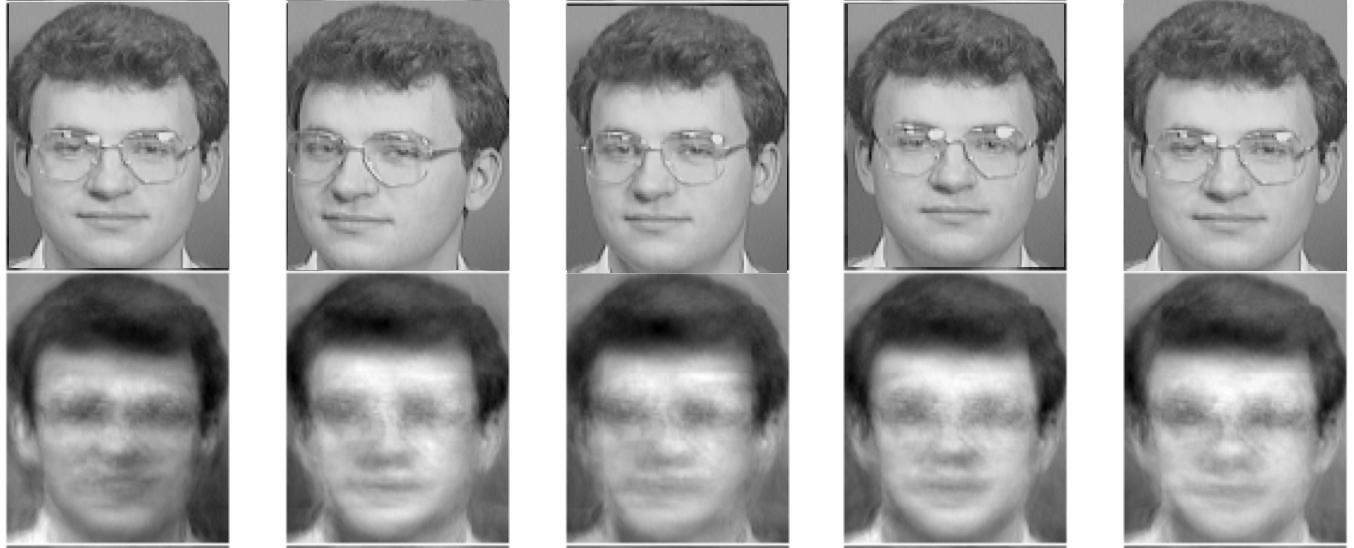
\includegraphics[scale=0.3]{img/eigenfaces.png}
\caption{Visages référents et les Eigenfaces correspondants}
\end{figure}


\begin{figure}[H]
\centering
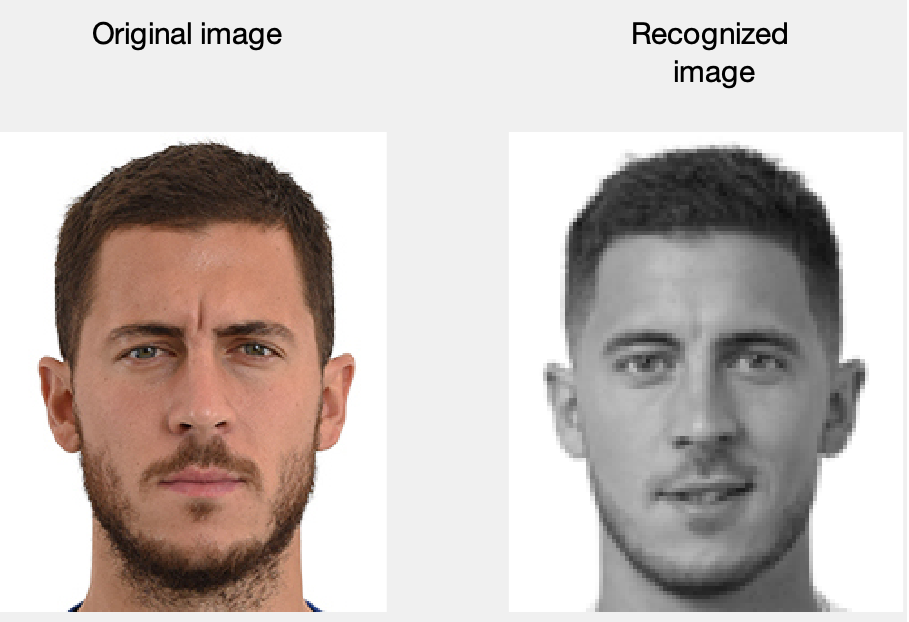
\includegraphics[scale=0.5]{img/recognition.png}
\caption{Exemple de reconnaissance faciale grâce à Eigenfaces}
\end{figure}

\section{VRecognition : SOM}
Dans cette partie encore en cours de développement, nous voulions utiliser le principe de SOM aussi connu comme « carte auto adaptative » pour reconnaitre un visage au sein d’une photo. Voici le fonctionnement. Tout d’abord, nous avons réalisé un traqueur de visage qui place un carré au-dessus du visage de la personne. Pour cela nous avons utilisé une toolbox Matlab pour detecter le visage plus facilement. Ensuite nous plaçons sur le visage 100 points. Si le visage bouge relativement lentement, les points suivent le visage. Cependant, si le visage bouge trop vite ou que quelque chose vient a cacher le visage, les points sont perdus. Pour éviter de perdre la trace d’un visage ainsi, nous recréons des points toutes les 10 frames afin de s’assurer qu’il y ait constamment 100 points sur le visage. Cela permet de suivre le visage avec une efficacité quasi-parfaite. La suite était nettement plus compliquée et nous a énormément retardé. Nous voulions utiliser l’algorithme de SOM ainsi : pour chaque nouveau visage, on prend 8 photos a intervalle de temps régulier. Puis on demande a l’utilisateur d’entrer le nom de la personne. On rogne la photo pour m’avoir que le visage et on transmet cette photo a notre carte auto adaptative. A partir de la, on utilise les 8 photos pour créer une carte auto adaptative unique, représentant le visage de la personne. Lorsqu’il faut reconnaitre le visage d’une personne, il n’y a plus qu’a mesurer la distance euclidienne entre chaque pixel de l’image (du visage a reconnaitre) avec chaque carte auto adaptative de la base de données. Plus l’image se rapproche d’une certaine carte auto adaptative, plus on peut penser qu’il s’agit d’une seule et meme personne. Pour pouvoir signaler qu’une personne n’existe pas dans la base de données, on peut également imposer un seuil de validité. Si la carte auto adaptative la plus proche et la photo n’ont qu’un pourcentage de ressemblance très faible, ou inférieur a 70\%, on peut penser qu’il ne s’agit pas de la bonne personne et donc que la personne n’existe pas dans la base de données. Malheureusement, nous avons commence a implementer SOM en c pour ensuite appeler la fonction depuis Matlab, mais pris par le temps nous avons  délaisser cette idée.


\end{document}